\documentclass{article}

\usepackage[utf8]{inputenc}
\usepackage[T1]{fontenc}
\usepackage[francais]{babel}
\usepackage{graphicx}

\begin{document}
\title{Algorithmes génétiques et application au problème du voyageur de commerce}
\author{Fabien Dubois\\
   Antoine RATO,\\
   Corentin HEMBISE	\\}
\date{\today}

\maketitle

\tableofcontents

\section{Principe des algorithmes génétiques}
	\subsection{Introduction}
	Les algorithmes génétiques sont des algorithme qui se basent sur la sélection naturelle afin de trouver des solutions à un problème d'optimisation. 

	La sélection naturelle est un processus de l'évolution des espèces. Les individus les plus adaptés à leur environnement, sont plus susceptible de « survivre », alors au fil de nouvelles générations, la population devient meilleur au regard de son environnement.

	En clair, les algorithmes génétique mime le processus de sélection naturelle pour trouver des solutions effocaces à un problème a un ou plusieurs paramètres.
	Les algorithmes génétiques sont des algorithmes d'approximation puisqu'il ne permettent pas de trouver la solution optimale à un problème, mais de s'en rapprocher. En outre, ils ont l'avantage de trouver une solution en un temps bien inférieur aux algorithmes déterministes.

	Quelques définitions :
	Les termes utilisés dans ce genre de problème sont empruntés de la génétique, ainsi, on parlera :
	\begin{description}
	\item [d'individu :] c'est une solution admissible du problème
	\item [de population :] c'est un ensemble d'individus
	\item [de gène :] c'est une partie d'un individu, une partie du problème
	\item [de génération :] c'est une itération de l'algorithme
	\item [de fonction objectif :] c'est une fonction qui permet de définir qu'un individu est meilleur qu'un autre
	\end{description}

	Pourquoi utiliser des algorithmes génétiques ?

	Dans les problèmes d'optimisation où le nombre de variables est grand, 

	\subsection{Principe}
	Les algorithmes de génétique se décomposent en 4 phases :
	\begin{itemize}
	\item La création d'une population initiale
	\item L'évaluation des individus
	\item La sélection, les croisement et les mutations
	\item (Éventuellement une nouvelle évaluation)
	\item La création d'une nouvelle population
	\end{itemize}

	\begin{figure}
		\begin{center}
			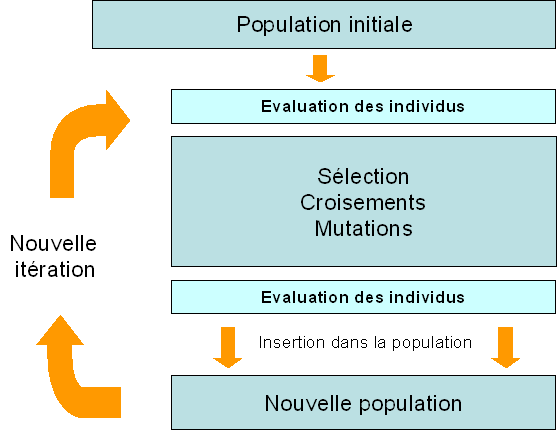
\includegraphics[scale=0.5]{schema_gen.png}
		\end{center}

		\caption{Schéma général d'un algorithme génétique}

		\label{Schéma général d'un algorithme génétique}
	\end{figure}


		\subsubsection{Population initiale}
		\subsubsection{Nouveau individus}

\section{Application au porblème du voyageur de commerce}
	\subsection{Définition du problème}
	Le problème est le suivant : 
	\begin{quote}
	Un voyageur de commerce doit visiter $n$ villes données en passant par chaque ville exactement une fois. Il commence par une ville quelconque et termine en retournant à la ville de départ.\\
	Quel chemin faut-il choisir afin de minimiser la distance parcourue ?
	\end{quote}
	
	\subsection{Modélisation du problème}
	
	Pour modéliser le problème, on définit un graphe complet dont les sommets sont les villes et les arrêtes sont éttiquetés par les distances entre les villes. Un chemin est définit par une permutation des entiers de 1 à n.
	Résoudre ce problème en trouvant une solution optimale reviendrais à parcourir l'ensemble des solutions du problème. C'est à dire l'ensemble de ces permutations, soit $n!$ \\
	Par exemple, pour 10, 30 et 100 villes : \\
	\begin{tabular}{cc}
	\hline
	$n$ & nombre de permutations \\
	\hline
	10 & 3 628 800 \\
	30 & $26 \times 10^{31}$ \\
	100 & $93 \times 10^{156}$ \\
	\hline
	\end{tabular}

	
	Un individu : un chemin, c'est à dire une permutation des entier de 1 à n
	Une ville sera représentée par un entier
	La fonction objectif à minimiser : calcule pour chaque chemin, la distance à parcourir

	\subsection{Modélisation du problème}

\section{Résultats}
	\subsection{Paramètrage de l'algorithme}

	Liste des paramètres sur lesquels influer :
	\begin{itemize}
	\item Nombre d'individus initial $]1,1000[$
	\item Nombre d'itérations max $]1,5000[$
	\item Nombre de villes $]10,50[$
	\item Méthode de selection (Elistisme, roulette, rang, tournoi)
	\item Taux de croisement $]0,1[$
	\item Taux de mutations $]0,1[$
	\item Taux de selection $]0,1[$
	\end{itemize}

	\subsection{Résultats}

\end{document}